\documentclass[11pt,a4paper]{article}

\usepackage[T1]{fontenc}
\usepackage[utf8]{inputenc}
\usepackage[italian]{babel}
\usepackage{amsmath,amssymb}
\usepackage[a4paper,margin=2.5cm]{geometry}
\usepackage{array}
\usepackage{siunitx}
\usepackage{booktabs}
\usepackage{graphicx}
\usepackage{float}
\usepackage{hyperref}

\hypersetup{hidelinks}
\setlength{\parindent}{0pt}
\setlength{\parskip}{4pt}
\allowdisplaybreaks
\graphicspath{{figure/}}
\sisetup{output-decimal-marker={,}, group-separator={\,}, per-mode=symbol,
         exponent-product=\cdot, range-phrase={\text{--}}}

\newcommand{\uma}{u-a}
\newcommand{\upa}{u+a}
\newcommand{\Mr}{M_{r}}
\newcommand{\fa}{f_a}

\title{Gasdinamica -- Svolgimento esercizio 2\\[2pt]
\large Urto piano contro una brusca riduzione d'area}
\author{}
\date{Prova di settembre 2022}

\begin{document}
\maketitle

\section*{Traccia}
Un'onda d'urto piana a $M=3$ propaga in aria in quiete [$\rho_0=\SI{1.29}{kg/m^3}$, $p_0=\SI{1}{atm}$] lungo
un condotto assialsimmetrico nel quale è presente una brusca riduzione dell'area della sezione.
Nell'interazione con la variazione d'area l'urto subisce un fenomeno di riflessione-trasmissione e questo a
sua volta induce la nascita di altre onde. Nelle figure sono riportati i valori assunti lungo il condotto per
diversi istanti di tempo dal numero di Mach e dal fattore di amplificazione
\[
  \fa=\frac{p_5-p_0}{p_1-p_0}.
\]
Fornire una ricostruzione delle caratteristiche principali del flusso generato dall'interazione tra urto e
variazione di sezione. Descrivere il fenomeno nel piano $x$--$t$. (Valutazione 9/30.)

\begin{figure}[H]
  \centering
  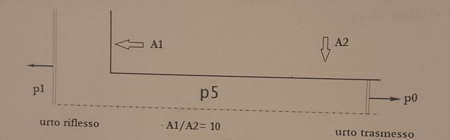
\includegraphics[width=0.72\textwidth]{schema.png}
  \caption{Schema della traccia: condotto largo $A_1$ a sinistra, condotto stretto $A_2$ a destra,
  $A_1/A_2=10$; urto riflesso verso sinistra (davanti a esso $p_1$), urto trasmesso verso destra nel gas in
  quiete $p_0$, pressione $p_5$ nel condotto stretto.}
  \label{fig:schema}
\end{figure}

%==============================================================================
\section{Lettura del testo e dati}
L'urto incidente viaggia verso destra nel condotto largo $A_1$ e incontra il salto d'area verso il condotto
stretto $A_2=A_1/10$. Dallo schema leggo le etichette: $p_0$ è il gas in quiete, $p_1$ è lo stato dietro
l'urto incidente (cioè davanti all'urto riflesso, che risale verso sinistra), $p_5$ è lo stato dietro l'urto
trasmesso nel condotto stretto. Il fattore $\fa$ confronta quindi la sovrappressione dell'urto trasmesso con
quella dell'incidente: $\fa>1$ significa urto amplificato.

Si chiede di ricostruire le onde nate dall'interazione, i loro stati e la loro evoluzione nel piano $x$--$t$.
Le figure con l'andamento di $M$ e di $\fa$ lungo il condotto non sono riportate nella copia della traccia: le
ricostruisco con il modello (\S\,\ref{sec:rappr}).

\begin{table}[H]
  \centering
  \begin{tabular}{lll}
    \toprule
    Grandezza & Valore & Note \\
    \midrule
    $\gamma$, $R$ & $\num{1.4}$, \SI{287}{J/(kg.K)} & aria, gas perfetto \\
    $p_0$ & \SI{1}{atm} $=\SI{101325}{Pa}$ & gas in quiete, $u_0=0$ \\
    $\rho_0$ & \SI{1.29}{kg/m^3} & \\
    $a_0=\sqrt{\gamma p_0/\rho_0}$ & \SI{331.6}{m/s} & $T_0=p_0/(\rho_0R)=\SI{273.7}{K}$ \\
    $M_s$ & 3 & Mach dell'urto incidente (relativo al gas in quiete) \\
    $A_1/A_2$ & 10 & riduzione brusca \\
    \bottomrule
  \end{tabular}
\end{table}

%==============================================================================
\section{Modello e ipotesi}
\begin{itemize}
  \item \textbf{Quasi-1D instazionario, non viscoso, gas perfetto con $\gamma=\num{1.4}$.} Il condotto è
    assialsimmetrico e lontano dal salto d'area la sezione è costante: le onde sono piane e le grandezze sono
    medie sulla sezione. In ciascun tratto vale Eulero 1D (onde $\uma$, $u$, $\upa$, invarianti di Riemann nelle
    regioni continue, Rankine--Hugoniot attraverso gli urti). Le temperature raggiunte (fino a circa
    \SI{1250}{K}) rendono $\gamma$ costante un'approssimazione accettabile.
  \item \textbf{Brusca variazione d'area come discontinuità attraversata in modo stazionario.} La lunghezza
    del raccordo è trascurabile rispetto ai cammini delle onde e il tempo d'adattamento ($\sim D/a$) è
    trascurabile rispetto ai tempi di interesse: fra la sezione $A_1$ e la sezione $A_2$ si conservano portata,
    entalpia totale ed entropia (contrazione accelerante, perdite trascurate):
    \[
      \rho u A=\text{cost.},\qquad h+\frac{u^2}{2}=\text{cost.},\qquad \frac{p}{\rho^\gamma}=\text{cost.},
    \]
    cioè la legge delle aree fra le due sezioni con $p^0$ e $T^0$ uguali.
  \item \textbf{Problema autosimile.} Tutte le onde nascono nell'istante e nel punto in cui l'urto raggiunge il
    salto d'area (origine del piano $x$--$t$): a ciascun lato del salto la soluzione è una sequenza di stati
    uniformi, urti, contatti e ventagli centrati. Il modello descrive il campo asintotico, dopo il transitorio
    bidimensionale nell'intorno del salto (discusso al \S\,\ref{sec:disc}).
\end{itemize}

%==============================================================================
\section{Analisi qualitativa}
\textbf{Stato dietro l'incidente.} Per $M_s=3$ il gas investito si muove verso destra con velocità
\emph{supersonica} (lo verifico subito al \S\,\ref{sec:calcolo}, $M_1\approx\num{1.36}$). Una corrente
stazionaria supersonica con $M_1=\num{1.36}$ può attraversare una contrazione solo se $A_1/A_2\le A/A^*(M_1)
\approx\num{1.09}$: con $A_1/A_2=10$ la corrente 1 non può entrare così com'è nel condotto stretto.

\textbf{Onda riflessa.} Il salto d'area si comporta per il 90\,\% della sezione come una parete: il gas 1
viene frenato e nasce una compressione della famiglia $\uma$ che risale verso sinistra. Poiché la corrente 1
è supersonica, l'informazione può risalirla solo con un \textbf{urto} ($|\Mr|>1$ rispetto al gas 1), che
rende subsonico lo stato 2 a valle. Riflessione con la stessa natura dell'incidente, come su una parete.

\textbf{Sezione $A_2$ sonica.} Lo stato 2, subsonico e ad alta pressione, accelera nella contrazione verso un
condotto stretto inizialmente a \SI{1}{atm}: la forte differenza di pressione porta la sezione $A_2$ in
condizioni critiche ($M=1$), come la gola di un ugello alimentato da un serbatoio. L'ipotesi va verificata a
posteriori con la natura dell'onda $\uma$ nel condotto stretto.

\textbf{Onde nel condotto stretto.} Il gas che entra in $A_2$ fa da pistone sul gas in quiete: nasce un
\textbf{urto trasmesso} $\upa$ verso destra e, fra il gas entrato (che ha attraversato due urti) e quello che
era già nel condotto stretto (un solo urto), un \textbf{contatto}. Per raccordare lo stato sonico in $A_2$
con lo stato dietro l'urto trasmesso serve un'onda $\uma$: se è un'espansione il gas accelera oltre la
velocità del suono e la sua testa ($u-a=0$) resta ferma nella sezione $A_2$, coerentemente con la sezione
sonica. Mi aspetto un urto trasmesso più forte dell'incidente, perché in un condotto che si restringe
un'onda di compressione si intensifica.

%==============================================================================
\section{Topologia del campo}
Il campo è autosimile con centro nell'origine ($x=0$ salto d'area, $t=0$ arrivo dell'urto), figura~\ref{fig:xt}.
\begin{itemize}
  \item $t<0$: stato 0 (quiete) davanti all'urto incidente, stato 1 dietro.
  \item Condotto largo, $t>0$: stato 1 | \textbf{urto riflesso} $\uma$ (velocità $W_r<0$) | stato 2,
    uniforme fino alla sezione $x=0^-$.
  \item Salto d'area: collegamento stazionario $2\to3$, con lo stato 3 sonico nella sezione $x=0^+$.
  \item Condotto stretto: \textbf{espansione centrata $\uma$} con testa verticale ($u_3-a_3=0$) e coda
    $u_4-a_4>0$ | stato 4 | \textbf{contatto} ($u^*$) | stato 5 | \textbf{urto trasmesso} $\upa$ ($W_t$) |
    stato 0.
\end{itemize}
Non ci sono zone d'interazione a due famiglie: oltre agli stati uniformi c'è un solo ventaglio, un'onda
semplice con caratteristiche $\uma$ semirette. Lo stato 3 occupa solo la sezione d'ingresso del condotto
stretto.

%==============================================================================
\section{Bilancio equazioni/incognite}
Dati gli stati 0 e 1, le incognite sono le intensità delle tre onde: urto riflesso ($\Mr$), onda $\uma$ nel
condotto stretto e urto trasmesso ($W_t$). Le equazioni sono la condizione di sezione sonica $M_3=1$ e le due
condizioni di contatto $p_4=p_5$, $u_4=u_5$: tre equazioni per tre incognite.
Se la sezione $A_2$ non fosse sonica, lo stato 3 sarebbe subsonico, non esisterebbe l'onda $\uma$ separata
nel condotto stretto e resterebbero due incognite ($\Mr$, $W_t$) con le due condizioni di contatto.

%==============================================================================
\section{Scorciatoie fisiche}
Con $A_2$ sonica, $A_2=A^*$ e il Mach nel condotto largo dietro il riflesso si legge dalla legge delle aree
senza conoscere il condotto stretto: $A_1/A^*=10$. Il problema si \textbf{disaccoppia}: l'urto riflesso
dipende solo da $M_2$, e il condotto stretto diventa un problema di Riemann con stato sinistro 3 noto.
Inoltre $M_2$ risulta molto piccolo, quindi il primo tentativo per l'urto riflesso è la riflessione su
parete chiusa ($u_2=0$).

%==============================================================================
\section{Calcolo}\label{sec:calcolo}

\subsection{Stato 1 (dietro l'urto incidente)}
Relazioni di salto con $M_s=3$:
\[
  \frac{p_1}{p_0}=\frac{2\gamma M_s^2-(\gamma-1)}{\gamma+1}=\frac{\num{2.8}\cdot9-\num{0.4}}{\num{2.4}}=\num{10.33},
\]
\[
  \frac{\rho_1}{\rho_0}=\frac{(\gamma+1)M_s^2}{(\gamma-1)M_s^2+2}=\frac{\num{21.6}}{\num{5.6}}=\num{3.857},
  \qquad \frac{T_1}{T_0}=\num{2.679}.
\]
\[
  W_i=M_sa_0=\SI{994.8}{m/s},\qquad u_1=W_i\left(1-\frac{\rho_0}{\rho_1}\right)=\SI{736.9}{m/s},\qquad
  a_1=a_0\sqrt{T_1/T_0}=\SI{542.8}{m/s},
\]
\[
  p_1=\SI{10.33}{atm},\quad \rho_1=\SI{4.98}{kg/m^3},\quad T_1=\SI{733}{K},\quad
  M_1=\frac{u_1}{a_1}=\num{1.358}>1 .
\]
Per $M_1=\num{1.358}$: $A/A^*=\num{1.093}\ll A_1/A_2=10$, quindi la corrente 1 non può attraversare la
contrazione: nasce l'urto riflesso.

\subsection{Stato 2 (dietro l'urto riflesso) con $A_2$ sonica}
Con $A_2=A^*$, la legge delle aree sul ramo subsonico dà
\[
  \frac{A_1}{A^*}=\frac1{M_2}\left[\frac{2}{\gamma+1}\left(1+\delta M_2^2\right)\right]^{\frac{\gamma+1}{2(\gamma-1)}}=10
  \quad\Rightarrow\quad M_2=\num{0.0580}.
\]
L'urto riflesso $\uma$ viaggia nel gas 1; il salto di velocità fissa il suo Mach relativo:
\[
  \Mr=X+\sqrt{1+X^2},\qquad X=\frac{\gamma+1}{4}\,\frac{u_1-u_2}{a_1},
  \qquad u_2=M_2\,a_2 .
\]
Poiché $a_2$ dipende da $\Mr$, si itera su $u_2$:
\begin{itemize}
  \item primo tentativo, riflessione su parete $u_2=0$: $X=\num{0.815}$, $\Mr=\num{2.104}$,
    $p_2/p_1=\num{5.00}$, $a_2=\SI{723.0}{m/s}$, da cui $u_2=M_2a_2=\SI{41.9}{m/s}$;
  \item secondo tentativo, $u_2=\SI{41.9}{m/s}$: $X=\num{0.768}$, $\Mr=\num{2.029}$, $a_2=\SI{710.1}{m/s}$,
    $u_2=\SI{41.2}{m/s}$, che cambia $u_2$ di meno di \SI{1}{m/s}: il valore è assestato.
\end{itemize}
\[
  \Mr=\num{2.031},\qquad \frac{p_2}{p_1}=\frac{2\gamma\Mr^2-(\gamma-1)}{\gamma+1}=\num{4.644},\qquad
  \frac{\rho_2}{\rho_1}=\frac{(\gamma+1)\Mr^2}{(\gamma-1)\Mr^2+2}=\num{2.712},
\]
\[
  p_2=\SI{48.0}{atm},\quad \rho_2=\SI{13.5}{kg/m^3},\quad a_2=\SI{710.3}{m/s},\quad T_2=\SI{1256}{K},\quad
  u_2=\SI{41.2}{m/s},
\]
\[
  W_r=u_1-\Mr a_1=\num{736.9}-\num{2.031}\cdot\num{542.8}=\SI{-365}{m/s}.
\]
L'urto riflesso risale il condotto largo a \SI{365}{m/s}.

\subsection{Stato 3 (sezione d'ingresso del condotto stretto, sonica)}
Fra 2 e 3 si conservano $p^0$ e $T^0$:
\[
  p^0_2=p_2\left(1+\delta M_2^2\right)^{\frac{\gamma}{\gamma-1}}=\SI{48.1}{atm},\qquad
  a^0_2=a_2\sqrt{1+\delta M_2^2}=\SI{710.5}{m/s},
\]
\[
  p_3=p^0_2\left(\frac{2}{\gamma+1}\right)^{\frac{\gamma}{\gamma-1}}=\num{0.5283}\cdot\num{48.1}=\SI{25.4}{atm},\qquad
  u_3=a_3=a^0_2\sqrt{\frac{2}{\gamma+1}}=\SI{648.6}{m/s},
\]
\[
  \rho_3=\SI{8.57}{kg/m^3},\qquad T_3=\SI{1047}{K}.
\]

\subsection{Condotto stretto: problema di Riemann fra 3 (sinistra) e 0 (destra)}
Il primo tentativo sulla velocità del contatto è quello isentropico:
\[
  z=\frac{a_0}{a_3}\left(\frac{p_3}{p_0}\right)^{\frac{\gamma-1}{2\gamma}}=\num{0.812},\qquad
  u^{(0)}=\frac{z\,(a_3+\delta u_3)-(a_0-\delta u_0)}{\delta(1+z)}=\SI{828}{m/s}.
\]
$u^{(0)}>u_3$: a sinistra un'espansione, che dà $p_{\rm sx}=p_3\bigl[1-\delta(u^{(0)}-u_3)/a_3\bigr]^{2\gamma/(\gamma-1)}=\SI{17.1}{atm}$;
$u^{(0)}>u_0$: a destra un urto, che dà $p_{\rm dx}=\SI{12.5}{atm}$. Correggendo $u$ con le pendenze delle due
curve, al secondo passo $u=\SI{900.0}{m/s}$ e $|p_{\rm sx}-p_{\rm dx}|/p\approx4\cdot10^{-6}$,
fisicamente zero. Configurazione RCS:
\[
  u^*=u_4=u_5=\SI{900}{m/s},\qquad p^*=p_4=p_5=\SI{14.4}{atm}.
\]
\textbf{Stato 4} (coda dell'espansione, $a+\delta u$ uniforme):
\[
  a_4=a_3-\delta(u^*-u_3)=\num{648.6}-\num{0.2}\cdot\num{251.3}=\SI{598.3}{m/s},\qquad
  p_4=p_3\left(\frac{a_4}{a_3}\right)^{7}=\SI{14.4}{atm},
\]
\[
  \rho_4=\SI{5.72}{kg/m^3},\quad T_4=\SI{891}{K},\quad M_4=\num{1.504};\qquad
  \text{testa } u_3-a_3=0,\quad \text{coda } u_4-a_4=\SI{302}{m/s}.
\]
\textbf{Stato 5} (dietro l'urto trasmesso, gas 0 messo in moto a $u^*$):
\[
  X=\frac{\gamma+1}{4}\frac{u^*}{a_0}=\num{1.628},\qquad M_t=X+\sqrt{1+X^2}=\num{3.54},\qquad
  \frac{p_5}{p_0}=\frac{2\gamma M_t^2-(\gamma-1)}{\gamma+1}=\num{14.4},
\]
\[
  W_t=M_ta_0=\SI{1174}{m/s},\qquad \rho_5=\SI{5.53}{kg/m^3},\quad T_5=\SI{922}{K},\quad M_5=\num{1.479}.
\]

\subsection{Fattore di amplificazione}
\[
  \fa=\frac{p_5-p_0}{p_1-p_0}=\frac{\num{14.45}-1}{\num{10.33}-1}=\num{1.44}.
\]
L'urto trasmesso è più forte dell'incidente: $M_s$ passa da 3 a $\num{3.54}$.

%==============================================================================
\section{Verifiche a posteriori}
\begin{itemize}
  \item Urto incidente: $M_s=3>1$, $s_1/s_0=\num{1.56}>1$. Verificata.
  \item Urto riflesso: $\Mr=\num{2.03}>1$ rispetto al gas 1, $s_2/s_1=\num{1.15}>1$, $W_r<0$: sta nel condotto
    largo. Verificata.
  \item Stato 2 subsonico ($M_2=\num{0.058}$, $u_2-a_2<0$): le caratteristiche $\uma$ dal salto d'area
    raggiungono l'urto riflesso, il collegamento stazionario con monte subsonico è lecito. Verificata.
  \item Collegamento stazionario: $\rho_2u_2A_1=\rho_3u_3A_2$ ($\num{5558}$ contro $\num{5557}$
    \si{kg/(s.m^2)} riferiti ad $A_2$) e $T^0_2=T^0_3$. Verificata.
  \item Sezione $A_2$ sonica: l'onda $\uma$ nel condotto stretto è un'espansione ($p_4<p_3$, $u_4>u_3$), il gas
    accelera oltre $M=1$. Con una compressione l'ipotesi sarebbe caduta. Verificata.
  \item Espansione tutta nel condotto stretto: testa $u_3-a_3=0$, coda $u_4-a_4=\SI{302}{m/s}>0$. Verificata.
  \item Ordine delle onde nel condotto stretto: $\SI{302}{m/s}<u^*=\SI{900}{m/s}<W_t=\SI{1174}{m/s}$. Verificata.
  \item Urto trasmesso: $M_t=\num{3.54}>1$, $s_5/s_0=\num{1.88}>1$. Verificata.
  \item Contatto: $p_4=p_5$, $u_4=u_5$, $\rho_4=\num{5.72}\ne\rho_5=\num{5.53}$; $a>0$ e $p>0$ ovunque. Verificata.
\end{itemize}

%==============================================================================
\section{Risultati}
\begin{table}[H]
  \centering
  \begin{tabular}{clrrrrrr}
    \toprule
    Stato & Posizione & $p$ [atm] & $\rho$ [kg/m$^3$] & $u$ [m/s] & $a$ [m/s] & $T$ [K] & $M$ \\
    \midrule
    0 & quiete & 1 & 1,29 & 0 & 332 & 274 & 0 \\
    1 & dietro l'incidente & 10,3 & 4,98 & 737 & 543 & 733 & 1,36 \\
    2 & dietro il riflesso ($A_1$) & 48,0 & 13,5 & 41 & 710 & 1256 & 0,058 \\
    3 & ingresso di $A_2$ & 25,4 & 8,57 & 649 & 649 & 1047 & 1 \\
    4 & coda dell'espansione & 14,4 & 5,72 & 900 & 598 & 891 & 1,50 \\
    5 & dietro il trasmesso & 14,4 & 5,53 & 900 & 609 & 922 & 1,48 \\
    \bottomrule
  \end{tabular}
\end{table}
\begin{table}[H]
  \centering
  \begin{tabular}{lll}
    \toprule
    Onda & Velocità nel piano $x$--$t$ & Intensità \\
    \midrule
    urto incidente $\upa$ & $W_i=\SI{995}{m/s}$ & $M_s=3$, $p_1/p_0=\num{10.3}$ \\
    urto riflesso $\uma$ & $W_r=\SI{-365}{m/s}$ & $\Mr=\num{2.03}$, $p_2/p_1=\num{4.64}$ \\
    espansione $\uma$ & testa 0, coda \SI{302}{m/s} & $p_4/p_3=\num{0.57}$ \\
    contatto & $u^*=\SI{900}{m/s}$ & $T_4=\SI{891}{K}$, $T_5=\SI{922}{K}$ \\
    urto trasmesso $\upa$ & $W_t=\SI{1174}{m/s}$ & $M_t=\num{3.54}$, $p_5/p_0=\num{14.4}$ \\
    \midrule
    \multicolumn{3}{l}{Fattore di amplificazione $\fa=(p_5-p_0)/(p_1-p_0)=\num{1.44}$} \\
    \bottomrule
  \end{tabular}
\end{table}

%==============================================================================
\section{Rappresentazioni}\label{sec:rappr}

\begin{figure}[H]
  \centering
  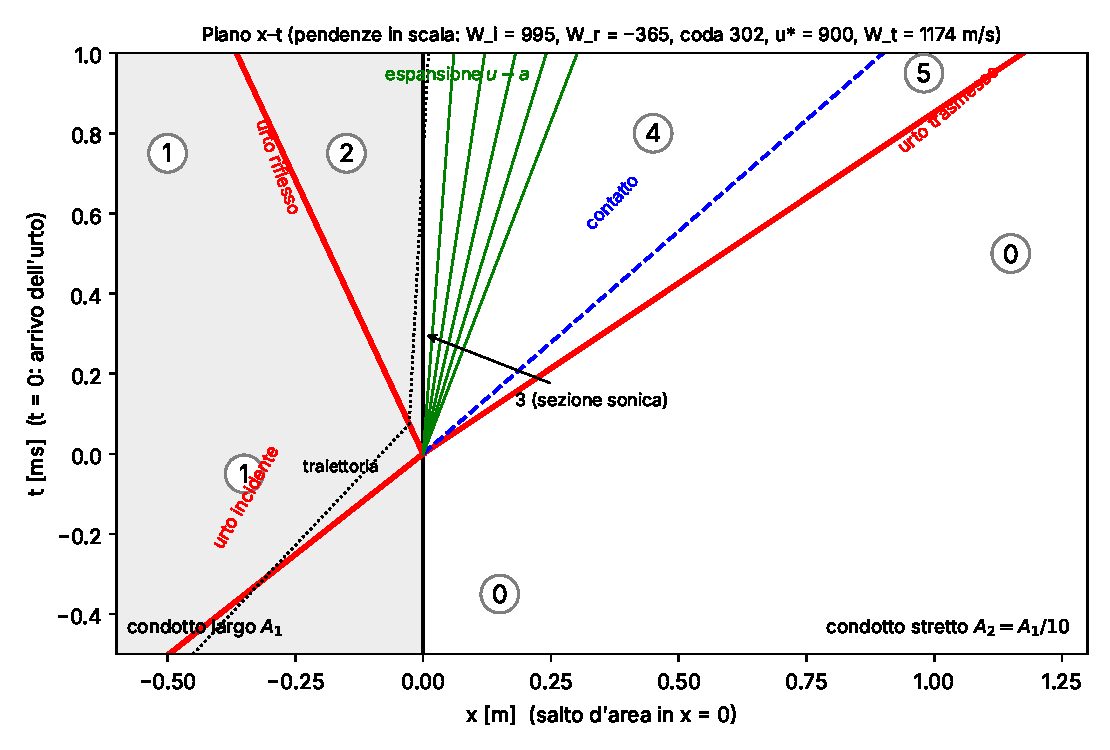
\includegraphics[width=0.85\textwidth]{xt.pdf}
  \caption{Piano $x$--$t$ con le pendenze calcolate (stati numerati; in grigio il condotto largo).}
  \label{fig:xt}
\end{figure}
\textbf{Piano $x$--$t$.} Prima di $t=0$ c'è solo l'urto incidente. All'arrivo nel salto d'area nascono, tutte
dall'origine: l'urto riflesso, che risale il condotto largo lasciando dietro di sé il gas 2 quasi fermo;
nel condotto stretto il ventaglio di espansione con la testa \emph{verticale}, incollata alla sezione
sonica, l'urto trasmesso e il contatto che separa il gas passato dal salto d'area (stati 3--4) dal gas che si
trovava già nel condotto stretto (stato 5). La traiettoria tratteggiata mostra una particella del condotto
largo: corre a \SI{737}{m/s}, viene quasi fermata dall'urto riflesso e poi si avvicina lentamente al salto
d'area, dove accelera fino a $M=1$ ed entra nel ventaglio.

\begin{figure}[H]
  \centering
  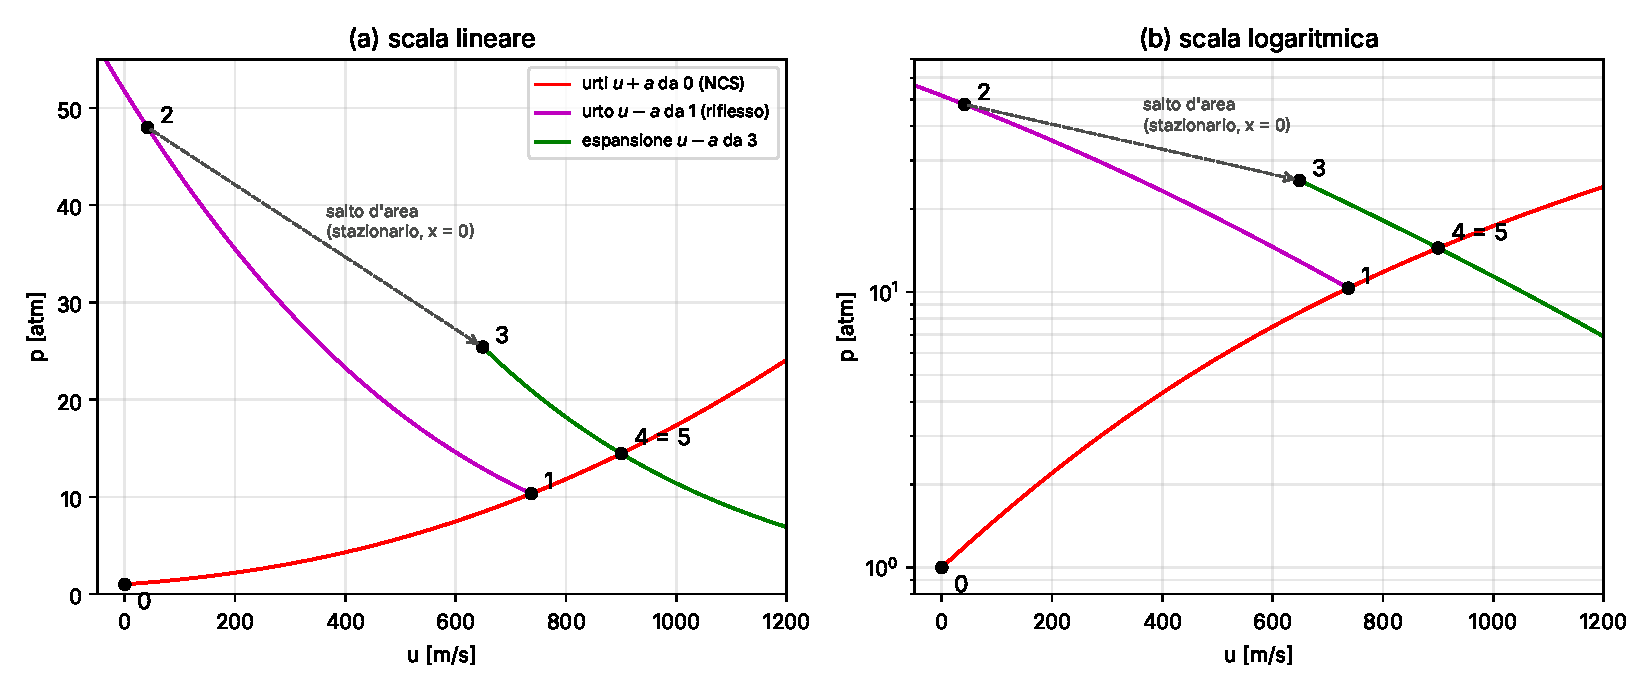
\includegraphics[width=\textwidth]{pu.pdf}
  \caption{Piano $p$--$u$ in scala lineare (a) e logaritmica (b). Il salto $2\to3$ non è un'onda ma il
  collegamento stazionario nella sezione $x=0$.}
  \label{fig:pu}
\end{figure}
\textbf{Piano $p$--$u$.} Le pressioni vanno da 1 a \SI{48}{atm}, quindi riporto entrambe le scale. Lo stato 1 sta
sulla curva degli urti $\upa$ uscente da 0 (urto incidente). Dal punto 1 lo stato 2 si trova risalendo la
curva dell'urto $\uma$ fino a $u_2\approx0$: è quasi il punto della riflessione su parete. Il salto
$2\to3$ avviene a $x$ fissato e non segue curve d'onda: abbassa la pressione e porta la velocità a quella del
suono. Dal punto 3 la curva di espansione $\uma$ incontra di nuovo la curva degli urti uscente da 0 nel punto
$4=5$, che sta sopra il punto 1: è l'amplificazione dell'urto. Il contatto non si vede nel piano $p$--$u$
($\rho_4\neq\rho_5$). La scala lineare mostra le distanze reali fra le pressioni, cioè quanto lo stato 2 è più
alto degli altri; quella logaritmica separa bene gli stati vicini a $p_0$ e rende leggibili i rapporti di
pressione delle singole onde.

\begin{figure}[H]
  \centering
  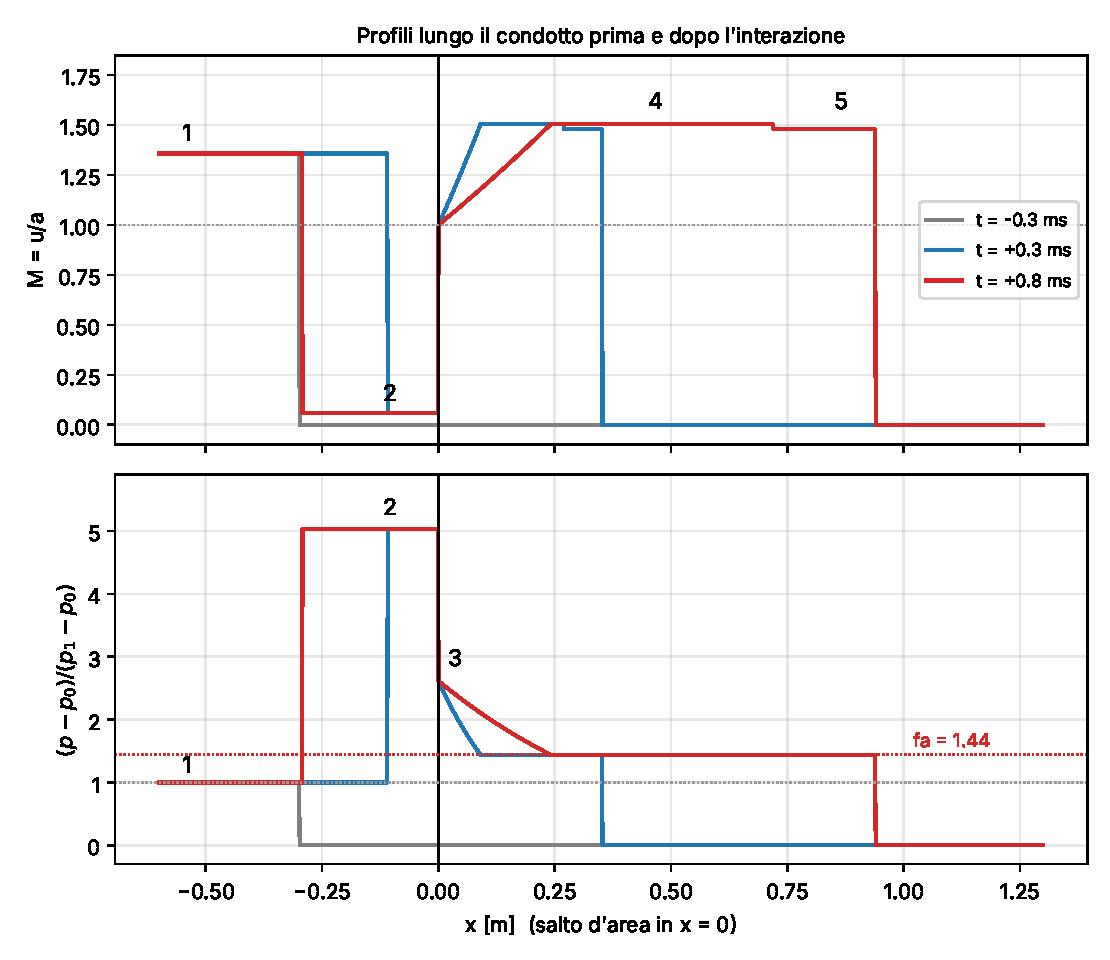
\includegraphics[width=0.85\textwidth]{profili.pdf}
  \caption{Numero di Mach e sovrappressione adimensionale $(p-p_0)/(p_1-p_0)$ lungo il condotto a tre istanti
  ($t<0$ prima dell'interazione).}
  \label{fig:profili}
\end{figure}
\textbf{Profili lungo il condotto.} Ricostruiscono le figure della traccia. Prima dell'interazione
($t=\SI{-0.3}{ms}$) c'è solo il gradino dell'urto incidente ($M=\num{1.36}$, sovrappressione unitaria). Dopo:
\begin{itemize}
  \item nel condotto largo il Mach crolla da \num{1.36} a \num{0.06} attraverso l'urto riflesso, mentre la
    sovrappressione sale a circa 5 volte quella dell'incidente;
  \item nel salto d'area il Mach sale a 1 e la sovrappressione scende a \num{2.6};
  \item nel ventaglio il Mach cresce da 1 a \num{1.50} e la pressione scende fino al plateau
    $\fa=\num{1.44}$, che si estende fino all'urto trasmesso;
  \item al contatto il Mach ha un piccolo salto ($\num{1.50}\to\num{1.48}$, perché $a_5>a_4$), mentre la
    pressione è continua.
\end{itemize}
Fra $t=\SI{0.3}{ms}$ e $t=\SI{0.8}{ms}$ i profili si allungano in proporzione al tempo senza cambiare valori:
è l'autosimilarità del modello, per cui $\fa$ resta costante.

%==============================================================================
\section{Discussione fisica}\label{sec:disc}
\textbf{Perché l'urto si amplifica.} Il salto d'area si comporta come la gola di un ugello alimentato da un
serbatoio: il gas 2, quasi fermo, ha $p^0\approx\SI{48}{atm}$ e $T^0\approx\SI{1256}{K}$ e scarica nel
condotto stretto in condizioni soniche. Il condotto stretto diventa un tubo d'urto con un ``driver'' più
caldo e a pressione più alta dello stato 1. Ne segue un urto trasmesso più forte dell'incidente ($\fa=\num{1.44}$,
$M_t=\num{3.54}$), come ci si aspetta da un'onda di compressione che entra in un condotto che si restringe.

\textbf{Peso del rapporto d'area.} Con $A_1/A_2=10$ il 90\,\% della sezione è parete: l'urto riflesso
($\Mr=\num{2.03}$, $p_2=\SI{48.0}{atm}$) è vicino a quello su parete chiusa ($\Mr=\num{2.10}$,
$p=\SI{51.7}{atm}$). Lo stesso modello dà $\fa\approx\num{1.20}$ per $A_1/A_2=2$ e $\fa\approx\num{1.52}$ per
$A_1/A_2\to\infty$, quindi con un rapporto 10 l'amplificazione è già vicina al suo limite. Ogni
contrazione con $A_1/A_2>\num{1.09}$ strozza la sezione $A_2$; solo sotto questo valore la corrente supersonica 1
passerebbe senza urto riflesso.

\textbf{Contatto.} Il gas 4 ha attraversato due urti ($M_s=3$ e $\Mr=\num{2.03}$) e un'espansione, il gas 5
un solo urto, più forte ($M_t=\num{3.54}$): il gas 5 ha più entropia ed è più caldo ($\SI{922}{K}$ contro
\SI{891}{K}). Il contatto è debole ma reale.

\textbf{Limiti del modello.} Nei primi istanti il campo è bidimensionale (assialsimmetrico): l'urto incidente
si riflette sulla corona del gradino, diffrange sullo spigolo d'ingresso del condotto stretto e l'urto
trasmesso è inizialmente curvo; diventa piano dopo qualche diametro del condotto stretto, e solo da lì valgono
i valori del modello quasi-1D. Allo spigolo vivo d'ingresso la corrente si separa (vena contratta) con perdite
di pressione totale: la sezione efficace è minore di $A_2$ e $p^0_3<p^0_2$, quindi $\fa$ reale è
un po' minore di \num{1.44}. Lontano dal salto lo strato limite nel condotto stretto attenua gradualmente
l'urto trasmesso.

\end{document}
